% one-figure manuscript written by fig_qc.py --tek-sekil-tex (trap T29)
\begin{figure}[!t]
\centering
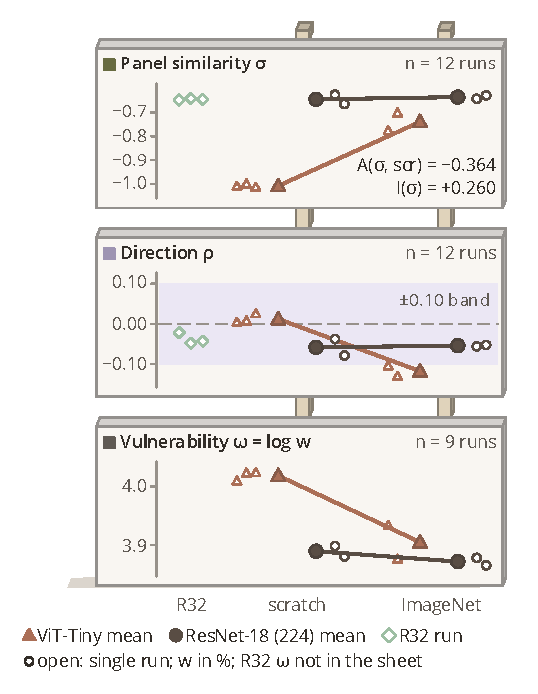
\includegraphics{fig9_cells_interaction}
\caption{\textbf{Two-by-two cells on CIFAR-10.} Panels Panel similarity σ, Direction ρ and Vulnerability ω share the initialization positions scratch and ImageNet; lines join cell means (split-half, log scale), open marks are runs, diamonds the R32 bridge. σ prints A(σ, scr) (H1) and I(σ) (H2); ρ carries the ±0.10 band. Each panel has its own scale.}
\label{fig:fig9_cells_interaction}
\end{figure}
